
\subsection{Presentation Layer}
Præsentationslaget i kasseapparatet er opbygget med XML i WPF. Selve laget blev først designet ved brug af skitsen på figur \ref{fig:KasseMockup} og derefter implementeret i visual studios WPF designer som set på figur \ref{fig:EndeligeGUI}. Da Grænsefladen var sat op så blev yderligere underliggende funktionalitet tilføjet såsom viewmodels. Disse vil blive forklaret i næste afsnit.

\begin{figure}[H]
	\centering
	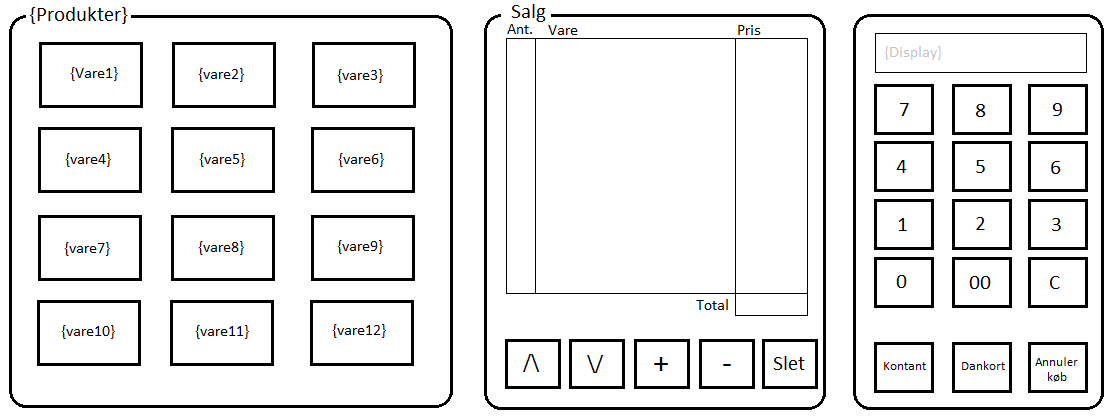
\includegraphics[width=1\textwidth]{Systemdesign/Frontend/pics/KasseMockup}
	\caption{Første mockup af grænsefladen til kasseapparatet.}
	\label{fig:KasseMockup}
\end{figure}

Denne skitse implementerede vi så.

\begin{figure}[H]
	\centering
	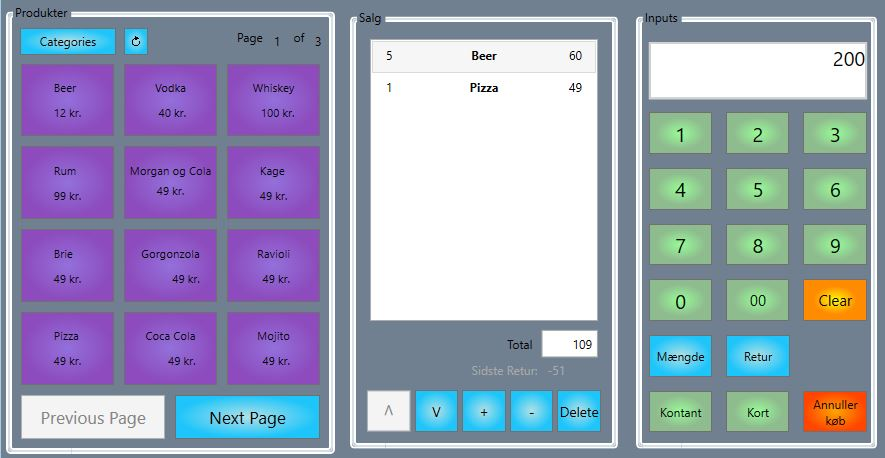
\includegraphics[width=1\textwidth]{Systemdesign/Frontend/pics/GUI}
	\caption{Den endelige grænseflade på kasseapparatet.}
	\label{fig:EndeligeGUI}
\end{figure}

Da grænsefladen var opsat var det nu nødvendigt at opsætte viewmodels til at forbinde grænsefladen med de underliggende lag.

\subsubsection{ViewModels}